
%%--------------------------------------------------
%% Customizations
%%--------------------------------------------------

%% http://www.texample.net/tikz/examples/periodic-table-of-chemical-elements/
\newcommand{\CommonElementTextFormat}[4]
{
  \begin{minipage}{2.2cm}
    \centering
      {\textbf{#1} \hfill #2}%
      \linebreak \linebreak
      {\textbf{#3}}%
      \linebreak \linebreak
      {{#4}}
  \end{minipage}
}

\newcommand{\NaturalElementTextFormat}[4]
{
  \CommonElementTextFormat{#1}{#2}{\Huge {#3}}{#4}
}

%%--------------------------------------------------
%% CPO: Multiple Choice Questions
%%--------------------------------------------------


%% Chapter 9: The Atom
%%--------------------------------------------------


%% Learning Objectives
%%--------------------------------------------------

%% Name the subatomic particles that make up an atom and describe their locations. 
%% Describe the forces that hold atoms together. 
%% Identify the number of particles in an atomic nucleus. 
%% Use the periodic table to obtain information about the elements. 
%% Explain the relationship between an elements placement on the periodic table and its chemical properties. 
%% Understand a simple model of electron arrangement. 
%% Explain the meaning of quantum theory. 
%% Compare and contrast the Bohr and quantum atomic models. 
%% Explain why probability is important when working with atom-sized systems.


%% CPO Multiple Choice Questions
%%--------------------------------------------------
\element{cpo-mc}{
\begin{question}{cpo-ch09-q01}
    The scientist published a detailed atomic theory in 1808 based on evidence he gathered through experiments with gases.
    His atomic theory laid the groundwork for later atomic models.
    \begin{multicols}{2}
    \begin{choices}
        \wrongchoice{James Chadwick}
      \correctchoice{John Dalton}
        \wrongchoice{Ernest Rutherford}
        \wrongchoice{J. J. Thomson}
    \end{choices}
    \end{multicols}
\end{question}
}

\element{cpo-mc}{
\begin{question}{cpo-ch09-q02}
    A common isotope of iron has a mass of 56.
    The total number of subatomic particles in the nucleon is:
    \begin{multicols}{4}
    \begin{choices}
        \wrongchoice{26}
      \correctchoice{56}
        \wrongchoice{30}
        \wrongchoice{4}
    \end{choices}
    \end{multicols}
\end{question}
}

\element{cpo-mc}{
\begin{question}{cpo-ch09-q03}
    The \rule[-0.1pt]{4em}{0.1pt} is one kind of particle that makes up the atom and carries a positive charge.
    \begin{multicols}{2}
    \begin{choices}
        \wrongchoice{electron}
      \correctchoice{proton}
        \wrongchoice{neutron}
        \wrongchoice{plasma}
    \end{choices}
    \end{multicols}
\end{question}
}

\element{cpo-mc}{
\begin{question}{cpo-ch09-q04}
    Atoms with the same atomic number but different atomic mass are called:
    \begin{multicols}{2}
    \begin{choices}
        \wrongchoice{prototypes.}
        \wrongchoice{isomers.}
      \correctchoice{isotopes.}
        \wrongchoice{ions.}
    \end{choices}
    \end{multicols}
\end{question}
}

\element{cpo-mc}{
\begin{question}{cpo-ch09-q05}
    The atomic number is the:
    \begin{choices}
        \wrongchoice{number of electrons plus the number of protons.}
        \wrongchoice{number of neutrons plus the number of protons.}
      \correctchoice{number of protons in the nucleus.}
        \wrongchoice{the average number of neutrons and protons for all naturally-occurring isotopes.}
    \end{choices}
\end{question}
}

\element{cpo-mc}{
\begin{question}{cpo-ch09-q06}
    Compared to protons, electrons have:
    \begin{choices}
      \correctchoice{much smaller mass and opposite charge.}
        \wrongchoice{about the same mass and opposite charge.}
        \wrongchoice{much larger mass and same charge.}
        \wrongchoice{Much larger mass and opposite charge.}
    \end{choices}
\end{question}
}

\element{cpo-mc}{
\begin{question}{cpo-ch09-q07}
    The electric charge of an atom with the same number of protons and electrons is:
    \begin{choices}
        \wrongchoice{equal to the number of protons multiplied by the charge of one proton.}
        \wrongchoice{equal to the number of electrons multiplied by the charge of one electron.}
        \wrongchoice{equal to the number of protons plus the number of neutrons.}
      \correctchoice{zero.}
    \end{choices}
\end{question}
}

\element{cpo-mc}{
\begin{question}{cpo-ch09-q08}
    The force that holds neutrons and protons together in the nucleus is known as:
    \begin{choices}
        \wrongchoice{the electromagnetic force}
        \wrongchoice{gravity}
      \correctchoice{the strong nuclear force}
        \wrongchoice{the weak nuclear force}
    \end{choices}
\end{question}
}

\element{cpo-mc}{
\begin{question}{cpo-ch09-q09}
    Protons and neutrons are found grouped together in the:
    \begin{multicols}{2}
    \begin{choices}
        \wrongchoice{electron cloud}
        \wrongchoice{charge}
      \correctchoice{nucleus}
        \wrongchoice{periodic table}
    \end{choices}
    \end{multicols}
\end{question}
}

\element{cpo-mc}{
\begin{question}{cpo-ch09-q10}
    Electrons are bound to the nucleus by:
    \begin{choices}
      \correctchoice{the electromagnetic force}
        \wrongchoice{gravity}
        \wrongchoice{the strong nuclear force}
        \wrongchoice{the weak nuclear force}
    \end{choices}
\end{question}
}

\element{cpo-mc}{
\begin{question}{cpo-ch09-q11}
    This scientist led a series of experiments that used high-speed positively-charged helium atoms to bombard very thin pieces of gold foil.
    Some of the helium atoms went straight through the foil, but a few bounced back.
    He used this information to hypothesize that an atom must be made of a tiny dense nucleus surrounded by a region of mostly empty space.
    \begin{multicols}{2}
    \begin{choices}
        \wrongchoice{James Chadwick}
        \wrongchoice{John Dalton}
      \correctchoice{Ernest Rutherford}
        \wrongchoice{J. J. Thomson}
    \end{choices}
    \end{multicols}
\end{question}
}

%% NOTE: do not like graphic
%\element{cpo-mc}{
%\begin{question}{cpo-ch09-q12}
%    Do any of the atom diagrams below represent atoms of the same element?
%    \begin{center}
%        \includegraphics[keepaspectratio,scale=0.8]{ch09-q12}
%    \end{center}
%    \begin{choices}
%        \wrongchoice{No, they are all different elements.}
%        \wrongchoice{Yes, atom $A$ and atom $B$ are the same element.}
%        \wrongchoice{Yes, all of the atoms are the same element.}
%      \correctchoice{Yes, atom $A$ and atom $C$ are the same element.}
%    \end{choices}
%\end{question}
%}

\element{cpo-mc}{
\begin{question}{cpo-ch09-q13}
    Which of the following is a \emph{true} statement about atoms?
    \begin{choices}
        \wrongchoice{All atoms of the same element have the same number of electrons, protons, and neutrons.}
        \wrongchoice{Atoms of different elements may have the same number of protons in the nucleus.}
      \correctchoice{All atoms of the same element have the same number of electrons and protons but may have different numbers of neutrons.}
        \wrongchoice{The number of neutrons is equal to the number of protons.}
    \end{choices}
\end{question}
}

\element{cpo-mc}{
\begin{question}{cpo-ch09-q14}
    Which of the following statements about two isotopes of the same element is \emph{false}?
    \begin{choices}
        \wrongchoice{The number of neutrons may be different between the two isotopes.}
        \wrongchoice{One isotope might be radioactive while the other isotope might be stable.}
        \wrongchoice{One isotope might have a larger mass than another isotope.}
      \correctchoice{The number of protons might be different between the two isotopes.}
    \end{choices}
\end{question}
}

\element{cpo-mc}{
\begin{question}{cpo-ch09-q15}
    The element chlorine has two stable isotopes,
        \ce{Cl^{35}} and \ce{Cl^{37}}.
    About 3 of every 4 chlorine atoms found on Earth are \ce{Cl^{35}},
        and the remainder are \ce{Cl^{37}}.
    The average atomic mass of chlorine is closest to:
    \begin{multicols}{2}
    \begin{choices}
        \wrongchoice{\SI{35}{\amu}}
      \correctchoice{\SI{35.5}{\amu}}
        \wrongchoice{\SI{36}{\amu}}
        \wrongchoice{\SI{36.5}{\amu}}
    \end{choices}
    \end{multicols}
\end{question}
}

\element{cpo-mc}{
\begin{question}{cpo-ch09-q16}
    The periodic table notation for carbon-13 (\ce{C^{13}}) is shown below.
    \begin{center}
    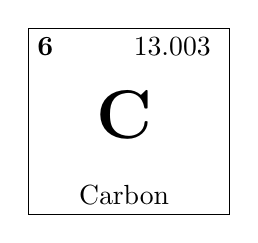
\begin{tikzpicture}
        \node[draw,rectangle] {\NaturalElementTextFormat{6}{13.003}{C}{Carbon}};
    \end{tikzpicture}
    \end{center}
    How many protons, electrons, and neutrons does carbon-13 have?
    \begin{multicols}{2}
    \begin{choices}
        \wrongchoice{6, 7, 13.}
      \correctchoice{6, 6, 7.}
        \wrongchoice{7, 6, 13.}
        \wrongchoice{7, 7, 13.}
    \end{choices}
    \end{multicols}
\end{question}
}

\element{cpo-mc}{
\begin{question}{cpo-ch09-q17}
    The periodic table notation for carbon-13 (\ce{C^{13}}) is shown below.
    \begin{center}
    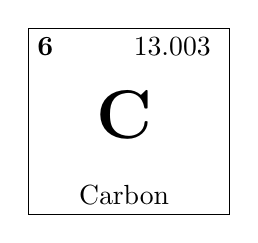
\begin{tikzpicture}
        \node[draw,rectangle] {\NaturalElementTextFormat{6}{13.003}{C}{Carbon}};
    \end{tikzpicture}
    \end{center}
    What is the mass number for carbon-13?
    \begin{multicols}{2}
    \begin{choices}
        %% NOTE: fixed error
        \wrongchoice{6}
        \wrongchoice{7}
        \wrongchoice{12}
      \correctchoice{13}
    \end{choices}
    \end{multicols}
\end{question}
}

\element{cpo-mc}{
\begin{question}{cpo-ch09-q18}
    The periodic table notation for silicon (\ce{Si}) is shown below.
    \begin{center}
    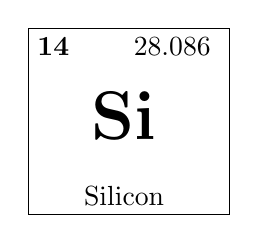
\begin{tikzpicture}
        \node[draw,rectangle] {\NaturalElementTextFormat{14}{28.086}{Si}{Silicon}};
    \end{tikzpicture}
    \end{center}
    An atom of silicon has how many electrons?
    \begin{choices}
      \correctchoice{14}
        \wrongchoice{7}
        \wrongchoice{28}
        \wrongchoice{cannot be determined with the information.}
    \end{choices}
\end{question}
}

\element{cpo-mc}{
\begin{question}{cpo-ch09-q19}
    all of the following are true for valence electrons \emph{except}:
    \begin{choices}
        \wrongchoice{valence electrons are in the highest energy level.}
        \wrongchoice{valence electrons determined almost all the properties of an element.}
        \wrongchoice{atoms may share or trade valence electrons.}
      \correctchoice{each element in the periodic table has a different number of valence electrons.}
    \end{choices}
\end{question}
}

\element{cpo-mc}{
\begin{question}{cpo-ch09-q20}
    The vertical columns of the periodic table are:
    \begin{multicols}{2}
    \begin{choices}
        \wrongchoice{periods}
      \correctchoice{groups}
        \wrongchoice{halogens}
        \wrongchoice{isotopes}
    \end{choices}
    \end{multicols}
\end{question}
}

\element{cpo-mc}{
\begin{question}{cpo-ch09-q21}
    A way of organizing the elements based on their chemical properties is the:
    \begin{multicols}{2}
    \begin{choices}
        \wrongchoice{energy level}
      \correctchoice{periodic table}
        \wrongchoice{nucleus}
        \wrongchoice{isotope}
    \end{choices}
    \end{multicols}
\end{question}
}

\element{cpo-mc}{
\begin{question}{cpo-ch09-q22}
    Most of the elements in the periodic table can be described as:
    \begin{multicols}{2}
    \begin{choices}
      \correctchoice{metals}
        \wrongchoice{nonmetals}
        \wrongchoice{metalloids}
        \wrongchoice{halogens}
    \end{choices}
    \end{multicols}
\end{question}
}

\element{cpo-mc}{
\begin{question}{cpo-ch09-q23}
    The noble gases such as helium and xenon do not form chemical bonds with other elements because they:
    \begin{choices}
      \correctchoice{have completely filled energy levels.}
        \wrongchoice{are chemically unstable.}
        \wrongchoice{are unusually large atoms.}
        \wrongchoice{have been around longest on the Earth.}
    \end{choices}
\end{question}
}

\element{cpo-mc}{
\begin{question}{cpo-ch09-q24}
    Which of the following statements about energy levels is \emph{true}?
    \begin{choices}
      \correctchoice{An energy level is a region in the electron cloud with a specific electron energy.}
        \wrongchoice{All energy levels must hold the same number of electrons.}
        \wrongchoice{The farther away an energy level is from the nucleus, the less energy is possesses.}
        \wrongchoice{Partially filled energy levels are more stable than completely filled energy levels.}
    \end{choices}
\end{question}
}

\element{cpo-mc}{
\begin{question}{cpo-ch09-q25}
    A group of students use a spectrometer to analyze three light sources.
    Different bright, vertical lines appear on the spectrometer scale as the light
        from each source enters the spectrometer.
    Each light source shows a different spectral pattern because:
    \begin{choices}
        \wrongchoice{all three light sources contain the same elements.}
      \correctchoice{there are different elements in each light source.}
        \wrongchoice{there are no elements associated with these light sources.}
        \wrongchoice{all elements have the same spectral pattern.}
    \end{choices}
\end{question}
}

%\element{cpo-mc}{
%\begin{question}{cpo-ch09-q26}
%    The diagram below shows a spectrum.
%    \begin{center}
%        %% NOTE: consider making a tikz diagram?
%        %% NOTE: this would be useful for texample
%        \includegraphics[keepaspectratio,scale=0.8]{ch09-q26}
%    \end{center}
%    The different colored bright lines represents:
%    \begin{choices}
%      \correctchoice{light of different energies.}
%        \wrongchoice{the diameter of atoms of different size.}
%        \wrongchoice{atoms that are radioactive.}
%        \wrongchoice{different values of the strong nuclear force.}
%    \end{choices}
%\end{question}
%}

\element{cpo-mc}{
\begin{question}{cpo-ch09-q27}
    A quanta is best described as:
    \begin{choices}
      \correctchoice{the smallest possible quantity of something.}
        \wrongchoice{A quanta of mass equals to one atom.}
        \wrongchoice{A particle of antimatter that releases enormous energy when it meets normal matter.}
        \wrongchoice{The result of adding one neutron, one proton, and one electron.}
    \end{choices}
\end{question}
}

\element{cpo-mc}{
\begin{question}{cpo-ch09-q28}
    Heisenburg's uncertainty principle tells us that:
    \begin{choices}
      \correctchoice{the act of observing in the quantum world changes the very system you are trying to measure.}
        \wrongchoice{we are always uncertain about the future of a particle.}
        \wrongchoice{atoms cannot exist with \SI{100}{\percent} probability.}
        \wrongchoice{quantum theory only applies to single atoms.}
    \end{choices}
\end{question}
}

\element{cpo-mc}{
\begin{question}{cpo-ch09-q29}
    Which of the following is evidence that electrons in atoms cannot have any amount of energy but instead are only allowed to have certain amounts of energy?
    \begin{choices}
        \wrongchoice{The atomic mass is the sum of the number of protons and neutrons.}
      \correctchoice{Only specific colors of light are given off by atoms.}
        \wrongchoice{All atoms of the same element have the same chemical properties.}
        \wrongchoice{Radioactive elements are unstable.}
    \end{choices}
\end{question}
}


\endinput


